\documentclass[a4paper]{report}
\usepackage[utf8]{inputenc}
\usepackage[T1]{fontenc}
\usepackage{RJournal}
\usepackage{amsmath,amssymb,array}
\usepackage{booktabs}


% tightlist command for lists without linebreak
\providecommand{\tightlist}{%
  \setlength{\itemsep}{0pt}\setlength{\parskip}{0pt}}


% Always define CSL refs as bib entries are contained in separate doc
% Pandoc citation processing
\newlength{\cslhangindent}
\setlength{\cslhangindent}{1.5em}
\newlength{\csllabelwidth}
\setlength{\csllabelwidth}{3em}
\newlength{\cslentryspacingunit} % times entry-spacing
\setlength{\cslentryspacingunit}{\parskip}
% for Pandoc 2.8 to 2.10.1
\newenvironment{cslreferences}%
  {}%
  {\par}
% For Pandoc 2.11+
\newenvironment{CSLReferences}[2] % #1 hanging-ident, #2 entry spacing
 {% don't indent paragraphs
  \setlength{\parindent}{0pt}
  % turn on hanging indent if param 1 is 1
  \ifodd #1
  \let\oldpar\par
  \def\par{\hangindent=\cslhangindent\oldpar}
  \fi
  % set entry spacing
  \setlength{\parskip}{#2\cslentryspacingunit}
 }%
 {}
\usepackage{calc}
\newcommand{\CSLBlock}[1]{#1\hfill\break}
\newcommand{\CSLLeftMargin}[1]{\parbox[t]{\csllabelwidth}{#1}}
\newcommand{\CSLRightInline}[1]{\parbox[t]{\linewidth - \csllabelwidth}{#1}\break}
\newcommand{\CSLIndent}[1]{\hspace{\cslhangindent}#1}


\usepackage{mathtools, longtable} \usepackage[ruled, linesnumbered]{algorithm2e} \usepackage{longtable}


\begin{document}


%% do not edit, for illustration only
\sectionhead{Contributed research article}
\volume{13}
\volnumber{2}
\year{2021}
\month{December}
\setcounter{page}{624}

\begin{article}
  % !TeX root = RJwrapper.tex
\title{Visual Diagnostics for Constrained Optimisation with Application to Guided Tours}
\author{by H. Sherry Zhang, Dianne Cook, Ursula Laa, Nicolas Langrené, and Patricia Menéndez}

\maketitle

\abstract{%
A guided tour helps to visualise high-dimensional data by showing low-dimensional projections along a projection pursuit optimisation path. Projection pursuit is a generalisation of principal component analysis in the sense that different indexes are used to define the interestingness of the projected data. While much work has been done in developing new indexes in the literature, less has been done on understanding the optimisation. Index functions can be noisy, might have multiple local maxima as well as an optimal maximum, and are constrained to generate orthonormal projection frames, which complicates the optimization. In addition, projection pursuit is primarily used for exploratory data analysis, and finding the local maxima is also useful. The guided tour is especially useful for exploration because it conducts geodesic interpolation connecting steps in the optimisation and shows how the projected data changes as a maxima is approached. This work provides new visual diagnostics for examining a choice of optimisation procedure based on the provision of a new data object which collects information throughout the optimisation. It has helped to diagnose and fix several problems with projection pursuit guided tour. This work might be useful more broadly for diagnosing optimisers and comparing their performance. The diagnostics are implemented in the R package \href{https://github.com/huizezhang-sherry/ferrn}{ferrn}.
}

\hypertarget{introduction}{%
\section{Introduction}\label{introduction}}

Visualisation is widely used in exploratory data analysis (Tukey 1977; Unwin 2015; Healy 2018; Wilke 2019). Presenting information in graphics often unveils insights that would otherwise not be discovered and provides a more comprehensive understanding of the problem at hand. Task-specific tools such as Li, Zhao, and Scheidegger (2020) show how visualisation can be used to understand, for instance, the behaviour of the optimisation for the example of neural network classification models. However, no general visualisation tool is available for diagnosing optimisation procedures. The work presented in this paper brings visualization tools into optimisation problems with the aim to better understand the performance of optimisers in practice.

The focus of this paper is on the optimisation problem arising in the projection pursuit guided tour (Buja et al. 2005), an exploratory data analysis technique used for detecting interesting structures in high-dimensional data through a set of lower-dimensional projections (Dianne Cook et al. 2008). The goal of the optimisation is to identify the projection, represented by the projection matrix, that gives the most interesting low-dimensional view. A view is said to be interesting if it can show some structures of the data that depart from normality, such as bimodality, clustering, or outliers.

The optimization challenges encountered in the projection pursuit guided tour problem are common to those of optimization in general. Examples include the existence of multiple optima (local and global), the trade-off between computational burden and proximity to the optima, or dealing with noisy objective functions that might be non-smooth and non-differentiable (Jones, Schonlau, and Welch 1998). The visualization tools, optimization methods, and conceptual framework presented in this paper can therefore be applied to other optimization problems.

The remainder of the paper is organised as follows. The next section provides an overview of optimisation methods, specifically random search and line search methods. A review of the projection pursuit guided tour, an overview of the optimisation problem and, outlines of three existing algorithms follows. The third section presents the new visual diagnostics, including the design of a data structure to capture information during the optimisation, from which several diagnostic plots are created. An illustration of how the diagnostic plots can be used to examine the performance of different optimisers and guide improvements to existing algorithms is shown using simulated data. Finally, an explanation of the implementation in the R package, \CRANpkg{ferrn} (Zhang et al. 2021), is provided.

\hypertarget{optim}{%
\section{Optimisation methods}\label{optim}}

The type of optimisation problem considered in this paper is constrained optimization (Bertsekas 2014), assuming it is not possible to find a solution to the problem in the way of a closed-form. That is, the problem consists in finding the minimum or maximum of a function \(f \in L^p\) in the constrained space \(\mathcal{A}\), where \(L^p\) defines the vector space of function \(f\), whose \(p\)th power is integrable.

Gradient-based methods are commonly used to optimise an objective function, with the most notable one being the gradient ascent (descent) method. Although these methods are popular, they rely on the availability of the objective function derivatives. As will be shown in the next section, the independent variables in our optimisation problem are the entries of a projection matrix, and the computational time required to perform differentiation on a matrix could impede the rendering of tour animation. In addition, some objective functions rely on the empirical distribution of the data, which makes it in general not possible to get the gradient. Hence, gradient-based methods are not the focus of this paper, and consideration will be given to derivative-free methods.

Derivative-free methods (Conn, Scheinberg, and Vicente 2009; Rios and Sahinidis 2013), which do not rely on the knowledge of the gradient, are more generally applicable. Derivative-free methods have been developed over the years, where the emphasis is on finding, in most cases, a near-optimal solution. Here we consider three derivative-free methods, two of which are random search methods: creeping random search and simulated annealing, and the other one is pseudo-derivative search.

Random search methods (Romeijn 2009; Zabinsky 2013; Andradóttir 2015) have a random sampling component as part of their algorithms and have been shown to have the ability to optimise non-convex and non-smooth functions. The initial random search algorithm, pure random search (Brooks 1958), draws candidate points from the entire space without using any information of the current position and updates the current position when an improvement on the objective function is made. As the dimension of the space becomes larger, sufficient sampling from the entire space would require a long time for convergence to occur, despite a guaranteed global convergence (Spall 2005). Various algorithms have thus been developed to improve pure random search by either concentrating on a narrower sampling space or using a different updating mechanism. Creeping random search (White 1971) is such a variation, where a candidate point is generated within a neighbourhood of the current point. This makes creeping random search faster to compute but global convergence is no longer guaranteed. On the other hand, simulated annealing (Kirkpatrick, Gelatt, and Vecchi 1983; Bertsimas and Tsitsiklis 1993), introduces a different updating mechanism. Rather than only updating the current point when an improvement is made, it uses a Metropolis acceptance criterion, where worse candidates still have a chance to be accepted. The convergence of simulated annealing algorithms has been widely researched (Mitra, Romeo, and Sangiovanni-Vincentelli 1986; Granville, Krivánek, and Rasson 1994) and the global optimum can be attained under mild regularity conditions.

The pseudo-derivative search uses a common search scheme in optimisation: line search. In line search methods, users are required to provide an initial estimate \(x_{1}\) and, at each iteration, a search direction \(S_k\) and a step size \(\alpha_k\) are generated. Then one moves on to the next point following \(x_{k+1} = x_k + \alpha_kS_k\) and the process is repeated until the desired convergence is reached. In derivative-free methods, local information of the objective function is used to determine the search direction. The choice of step size also needs consideration, as inadequate step sizes might prevent the optimisation method from converging to an optimum. An ideal step size can be chosen by finding the value of \(\alpha_k \in \mathbb{R}\) that maximises \(f(x_k + \alpha_kS_k)\) with respect to \(\alpha_k\) at each iteration.

\hypertarget{projection-pursuit-guided-tour}{%
\section{Projection pursuit guided tour}\label{projection-pursuit-guided-tour}}

A projection pursuit guided tour combines two different methods (projection pursuit and guided tour) to explore interesting features in a high-dimensional space. Projection pursuit, coined by Friedman and Tukey (1974), detects interesting structures (e.g., clustering, outliers, and skewness) in multivariate data via low-dimensional projections. Guided tour (Dianne Cook et al. 1995) is one variation of a broader class of data visualisation methods, tour (Buja et al. 2005), which displays high-dimensional data through a series of animated projections.

Let \(\mathbf{X}_{n \times p}\) be the data matrix with \(n\) observations in \(p\) dimensions. A \(d\)-dimensional projection is a linear transformation from \(\mathbb{R}^p\) into \(\mathbb{R}^d\) defined as \(\mathbf{Y} = \mathbf{X} \cdot \mathbf{A}\), where \(\mathbf{Y}_{n \times d}\) is the projected data and \(\mathbf{A}_{p\times d}\) is the projection matrix. We define \(f: \mathbb{R}^{n \times d} \mapsto \mathbb{R}\) to be an index function that maps the projected data \(\mathbf{Y}\) onto a scalar value. This is commonly known as the projection pursuit index function, or just index function, and is used to measure the ``interestingness'' of a given projection. An interesting projection shows structures that are non-normal since theoretical proofs from Diaconis and Freedman (1984) have shown that projections tend to be normal as \(n\) and \(p\) approach infinity under certain conditions. There have been many index functions proposed in the literature, here are a few examples: early indexes that can be categorised as measuring the \(L^2\) distance between the projection and a normal distribution: Legendre index (Friedman and Tukey 1974); Hermite index (Hall 1989); natural Hermite index (D. Cook, Buja, and Cabrera 1993); chi-square index (Posse 1995) for detecting spiral structure; LDA index (E. Lee et al. 2005) and PDA (E.-K. Lee and Cook 2010) index for supervised classification; kurtosis index (Loperfido 2020) and skewness index (Loperfido 2018) for detecting outliers in financial time series; and most recently, scagnostic indexes (Laa and Cook 2020) for summarising structures in scatterplot matrices based on eight scagnostic measures (L. Wilkinson, Anand, and Grossman 2005; Leland Wilkinson and Wills 2008).

As a general visualisation method, tour produces animations of high-dimensional data via rotations of low-dimensional planes. There are different versions depending on how the high-dimensional space is investigated: grand tour (Dianne Cook et al. 2008) selects the planes randomly to provide a general overview; manual tour (Dianne Cook and Buja 1997) gradually phases in and out one variable to understand the contribution of that variable in the projection. Guided tour, the main interest of this paper, chooses the planes with the aid of projection pursuit to gradually reveal the most interesting projection. Given a random start, projection pursuit iteratively finds bases with higher index values, and the guided tour constructs a geodesic interpolation between these planes to form a tour path. Figure \ref{fig:tour-path} shows a sketch of the tour path where the blue squares represent planes (targets) selected by the projection pursuit optimisation, and the white squares represent planes in the geodesic interpolation between targets. Mathematical details of the geodesic interpolation can be found in Buja et al. (2005). (Note that the term \emph{frame} used in Buja's paper refers to a particular set of orthonormal vectors defining a plane. This is also conventionally referred to as a basis, which is used in this paper and the associated software.) The aforementioned tour method has been implemented in the R package \CRANpkg{tourr} (H. Wickham et al. 2011).

\begin{figure}

{\centering \includegraphics[width=1\linewidth]{figs/tour-path} 

}

\caption{An illustration for demonstrating the frames in a tour path. Each square (frame) represents the projected data with a corresponding basis. Blue frames are returned by the projection pursuit optimisation and white frames are constructed between two blue frames by geodesic interpolation.}\label{fig:tour-path}
\end{figure}

\hypertarget{tour-optim}{%
\subsection{Optimisation in the tour}\label{tour-optim}}

In projection pursuit, the optimisation aims at finding the global and local maxima that give interesting projections according to an index function. That is, it starts with a given randomly selected basis \(\mathbf{A}_1\) and aims at finding an optimal final projection basis \(\mathbf{A}_T\) that satisfies the following optimisation problem:

\begin{align}
\arg \max_{\mathbf{A} \in \mathcal{A}} f(\mathbf{X} \cdot \mathbf{A})  ~~~ s.t. ~~~ \mathbf{A}^{\prime} \mathbf{A} = I_d \,,
\end{align}

\noindent where \(f\) and \(\mathbf{X}\) are defined as in the previous section, \(\mathcal{A}\) is the set of all \(p\)-dimensional projection bases, \(I_d\) is the \(d\)-dimensional identity matrix, and the constraint ensures the projection bases, \(\mathbf{A}\), to be orthonormal. It is worth noticing the following: 1) The optimisation is constrained, and the orthonormality constraint imposes a geometrical structure on the bases space: it forms a Stiefel manifold. 2) There may be index functions for which the objective function might not be differentiable. 3) While finding the global optimum is the goal of the optimisation problem, interesting projections may also appear in the local optimum. 4) The optimisation should be fast to compute since the tour animation is viewed by the users during the optimisation.

\hypertarget{existing-algorithms}{%
\subsection{Existing algorithms}\label{existing-algorithms}}

Three optimisers have been implemented in the \pkg{tourr} (H. Wickham et al. 2011) package: creeping random search (CRS), simulated annealing (SA), and pseudo-derivative (PD). Creeping random search (CRS) is a random search optimiser that samples a candidate basis \(\mathbf{A}_{l}\) in the neighbourhood of the current basis \(\mathbf{A}_{\text{cur}}\) by \(\mathbf{A}_{l} = (1- \alpha)\mathbf{A}_{\text{cur}} + \alpha \mathbf{A}_{\text{rand}}\) where \(\alpha \in [0,1]\) controls the radius of the sampling neighbourhood and \(\mathbf{A}_{\text{rand}}\) is generated randomly. \(\mathbf{A}_{l}\) is then orthonormalised to fulfil the basis constraint. If \(\mathbf{A}_{l}\) has an index value higher than the current basis \(\mathbf{A}_{\text{cur}}\), the optimiser outputs \(\mathbf{A}_{l}\) for a guided tour to construct an interpolation path. The neighbourhood parameter \(\alpha\) is adjusted by a cooling parameter: \(\alpha_{j+1} = \alpha_j * \text{cooling}\) before the next iteration starts. The optimiser terminates when the maximum number of iteration \(l_{\max}\) is reached before a better basis can be found. The algorithm of CRS can be found in the appendix. Posse (1995) has proposed a slightly different cooling scheme by introducing a halving parameter \(c\). In his proposal, \(\alpha\) is only adjusted if the last iteration takes more than \(c\) times to find a better basis.

Simulated annealing (SA) uses the same sampling process as CRS but allows a probabilistic acceptance of a basis with lower index value than the current one. Given an initial value of \(T_0 \in \mathbb{R^{+}}\), the ``temperature'' at iteration \(l\) is defined as \(T(l) = \frac{T_0}{\log(l + 1)}\). When a candidate basis fails to have an index value larger than the current basis, SA gives it a second chance to be accepted with probability \[P= \min\left\{\exp\left[-\frac{\mid I_{\text{cur}} - I_{l} \mid}{T(l)}\right],1\right\} \,,\] where \(I_{(\cdot)} \in \mathbb{R}\) denotes the index value of a given basis. This implementation allows the optimiser to make a move and explore the basis space even if the candidate basis does not have a higher index value. Hence it enables the optimiser to jump out of a local optimum. The second algorithm in the appendix highlights how SA differs from CRS in the inner loop.

Pseudo-derivative (PD) search uses a different strategy than CRS and SA. Rather than randomly sample the basis space, PD first computes a search direction by evaluating bases close to the current basis. The step size is then chosen along the corresponding geodesic by another optimisation over a 90 degree angle from \(-\pi/4\) to \(\pi/4\). The resulting candidate basis \(\mathbf{A}_{**}\) is returned for the current iteration if it has a higher index value than the current one. The third algorithm in the appendix summarises the inner loop of the PD.

\hypertarget{vis-diag}{%
\section{Visual diagnostics}\label{vis-diag}}

A data structure for diagnosing optimisers in projection pursuit guided tour is first defined. With this data structure, four types of diagnostic plots are presented.

\hypertarget{data-structure-for-diagnostics}{%
\subsection{Data structure for diagnostics}\label{data-structure-for-diagnostics}}

Three main pieces of information are recorded during the projection pursuit optimisation: 1) projection bases \(\mathbf{A}\), 2) index values \(I\), and 3) state \(S\). For CRS and SA, possible states include \texttt{random\_search}, \texttt{new\_basis}, and \texttt{interpolation}. Pseudo-derivative (PD) has a wider variety of states, including \texttt{new\_basis}, \texttt{direction\_search}, \texttt{best\_direction\_search}, \texttt{best\_line\_search}, and \texttt{interpolation}. Multiple iterators index the information collected at different levels: \(t\) is a unique identifier prescribing the natural ordering of each observation; \(j\) and \(l\) are the counter of the outer and inner loop, respectively. Other parameters of interest recorded, \(V\), include \texttt{method} that tags the name of the optimiser, and \texttt{alpha} that indicates the sampling neighbourhood size for searching observations. A matrix notation describing the data structure is:

\newpage

\begin{longtable}[]{@{}
  >{\raggedright\arraybackslash}p{(\columnwidth - 16\tabcolsep) * \real{0.0968}}
  >{\raggedright\arraybackslash}p{(\columnwidth - 16\tabcolsep) * \real{0.0968}}
  >{\raggedright\arraybackslash}p{(\columnwidth - 16\tabcolsep) * \real{0.0968}}
  >{\raggedright\arraybackslash}p{(\columnwidth - 16\tabcolsep) * \real{0.0968}}
  >{\raggedright\arraybackslash}p{(\columnwidth - 16\tabcolsep) * \real{0.0968}}
  >{\raggedright\arraybackslash}p{(\columnwidth - 16\tabcolsep) * \real{0.0968}}
  >{\raggedright\arraybackslash}p{(\columnwidth - 16\tabcolsep) * \real{0.0968}}
  >{\raggedright\arraybackslash}p{(\columnwidth - 16\tabcolsep) * \real{0.0968}}
  >{\raggedright\arraybackslash}p{(\columnwidth - 16\tabcolsep) * \real{0.2258}}@{}}
\toprule\noalign{}
\begin{minipage}[b]{\linewidth}\raggedright
\(t\)
\end{minipage} & \begin{minipage}[b]{\linewidth}\raggedright
\(\mathbf{A}\)
\end{minipage} & \begin{minipage}[b]{\linewidth}\raggedright
\(I\)
\end{minipage} & \begin{minipage}[b]{\linewidth}\raggedright
\(S\)
\end{minipage} & \begin{minipage}[b]{\linewidth}\raggedright
\(j\)
\end{minipage} & \begin{minipage}[b]{\linewidth}\raggedright
\(l\)
\end{minipage} & \begin{minipage}[b]{\linewidth}\raggedright
\(V_{1}\)
\end{minipage} & \begin{minipage}[b]{\linewidth}\raggedright
\(V_{2}\)
\end{minipage} & \begin{minipage}[b]{\linewidth}\raggedright
Description
\end{minipage} \\
\midrule\noalign{}
\endhead
\bottomrule\noalign{}
\endlastfoot
\(1\) & \(\mathbf{A}_1\) & \(I_1\) & \(S_1\) & 1 & 1 & \(V_{11}\) & \(V_{12}\) & start basis \\
\(2\) & \(\mathbf{A}_2\) & \(I_2\) & \(S_2\) & 2 & 1 & \(V_{21}\) & \(V_{22}\) & search \\
\ldots{} & \ldots{} & \ldots{} & \ldots{} & \ldots{} & \ldots{} & \ldots{} & \ldots{} & \ldots{} \\
\ldots{} & \ldots{} & \ldots{} & \ldots{} & 2 & \(l_2\) & \ldots{} & \ldots{} & search (accepted) \\
\ldots{} & \ldots{} & \ldots{} & \ldots{} & 2 & 1 & \ldots{} & \ldots{} & interpolation \\
\ldots{} & \ldots{} & \ldots{} & \ldots{} & \ldots{} & \ldots{} & \ldots{} & \ldots{} & \ldots{} \\
\ldots{} & \ldots{} & \ldots{} & \ldots{} & 2 & \(k_2\) & \ldots{} & \ldots{} & interpolation \\
\ldots{} & \ldots{} & \ldots{} & \ldots{} & \ldots{} & \ldots{} & \ldots{} & \ldots{} & \ldots{} \\
\ldots{} & \ldots{} & \ldots{} & \ldots{} & \(J\) & 1 & \ldots{} & \ldots{} & search \\
\ldots{} & \ldots{} & \ldots{} & \ldots{} & \ldots{} & \ldots{} & \ldots{} & \ldots{} & \ldots{} \\
\(T\) & \(\mathbf{A}_T\) & \(I_T\) & \(S_T\) & \(J\) & \(l_J\) & \(V_{T1}\) & \(V_{T2}\) & search (final) \\
\ldots{} & \ldots{} & \ldots{} & \ldots{} & \(J\) & 1 & \ldots{} & \ldots{} & interpolation \\
\ldots{} & \ldots{} & \ldots{} & \ldots{} & \ldots{} & \ldots{} & \ldots{} & \ldots{} & \ldots{} \\
\ldots{} & \ldots{} & \ldots{} & \ldots{} & \(J\) & \(k_J\) & \ldots{} & \ldots{} & interpolation \\
\ldots{} & \ldots{} & \ldots{} & \ldots{} & \(J+1\) & 1 & \ldots{} & \ldots{} & search (last round) \\
\ldots{} & \ldots{} & \ldots{} & \ldots{} & \ldots{} & \ldots{} & \ldots{} & \ldots{} & \ldots{} \\
\(T^{\prime}\) & \(\mathbf{A}_{T^{\prime}}\) & \(I_{T^{\prime}}\) & \(S_{T^{\prime}}\) & \(J+1\) & \(l_{J+1}\) & \(V_{{T}^{\prime}1}\) & \(V_{{T}^{\prime}2}\) & search (last round) \\
\end{longtable}

\noindent where \(T^{\prime} = T + k_{J}+ l_{J+1}\). Note that there is no output in iteration \(J + 1\) since the optimiser does not find a better basis in the last iteration and terminates. The final basis found is \(A_T\) with index value \(I_T\).

The data structure constructed above meets the tidy data principle (Hadley Wickham 2014) that requires each observation to form a row and each variable to form a column. With tidy data structure, data wrangling and visualisation can be significantly simplified by well-developed packages such as \CRANpkg{dplyr} (Hadley Wickham et al. 2020) and \CRANpkg{ggplot2} (Hadley Wickham 2016).

\hypertarget{diagnostic-1-checking-how-hard-the-optimiser-is-working}{%
\subsection{Diagnostic 1: Checking how hard the optimiser is working}\label{diagnostic-1-checking-how-hard-the-optimiser-is-working}}

A starting point of diagnosing an optimiser is to understand how many searches it has conducted, i.e., we want to summarise how the index is increasing over iterations and how many basis need to be sampled at each iteration. This is achieved using the function \texttt{explore\_trace\_search()}: a boxplot shows the distribution of index values for each try, where the accepted basis (corresponding to the highest index value) is always shown as a point. When there are only few tries at a given iteration, showing the data points directly is preferred over the boxplot and this is controlled via the \texttt{cutoff} argument. Additional annotations are added to facilitate better reading of the plot, and these include 1) the number of points searched in each iteration can be added as text label at the bottom of each iteration; 2) the anchor bases to interpolate are connected and highlighted in a larger size; 3) the colour of the last iteration is in greyscale to indicate no better basis found in this iteration.

Figure \ref{fig:toy-search} shows an example of the search plot for CRS (left) and SA (right). Both optimisers quickly find better bases in the first few iterations and then take longer to find one in the later iterations. The anchor bases, the ones found with the highest index value in each iteration, always have an increased index value in the optimiser CRS while this is not the case for SA. This feature gives CRS an advantage in this simple example to quickly find the optimum.

\begin{figure}

{\centering \includegraphics[width=1\linewidth]{figs/toy-search} 

}

\caption{A comparison of the searches by two optimisers: CRS (left) and SA (right) on a 2D projection problem of a six-variable dataset, \code{boa6} using the holes index. Both optimisers reach the final basis with a similar index value, while it takes SA longer to find the final basis. In the earlier iterations, optimisers quickly find a better basis to proceed, while in the later iterations, most sampled bases fail to make an improvement on the index value, and a boxplot is used to summarise the distribution of the index values. There is no better basis found in the last iteration, 9 (left) and 15 (right), before reaching the maximum number of try and hence it is coloured grey. The colour scale is from the customised botanical palette in the **ferrn** package.}\label{fig:toy-search}
\end{figure}

\hypertarget{toy-interp}{%
\subsection{Diagnostic 2: Examining the optimisation progress}\label{toy-interp}}

Another interesting feature to examine is the changes in the index value between interpolating bases since the projection on these bases is shown in the tour animation. Trace plots are created by plotting the index value against time. Figure \ref{fig:toy-interp} presents the trace plot of the same optimisations as Figure \ref{fig:toy-search}, and one can observe that the trace is smooth in both cases. It may seem bizarre at first sight that the interpolation sometimes passes bases with higher index values before it decreases to a lower target. This happens because, on the one hand, the probabilistic acceptance in SA implies that some worse bases will be accepted by the optimiser. In addition, the guided tour interpolates between the current and target basis to provide a smooth transition between projections, and sometimes a higher index value will be observed along the interpolation path. This indicates that a non-monotonic interpolation cannot be avoided, even for CRS. Later, in Section \emph{A problem of non-monotonicity}, there will be a discussion on improving the non-monotonic interpolation for CRS.

\begin{figure}

{\centering \includegraphics[width=1\linewidth]{figs/toy-interp} 

}

\caption{An inspection of the index values as the optimisation progress for two optimisers: CRS (left) and SA (right). The holes index is optimised for a 2D projection problem on the six-variable dataset \code{boa6}. Lines indicate the interpolation, and dots indicate new target bases generated by the optimisers. Interpolation in both optimisation is smooth, while SA is observed to first pass by some bases with higher index values before reaching the target bases in time 76-130.}\label{fig:toy-interp}
\end{figure}

\hypertarget{toy-pca}{%
\subsection{Diagnostic 3a: Understanding the optimiser's coverage of the search space}\label{toy-pca}}

Apart from checking the search and progression of an optimiser, looking at where the bases are positioned in the basis space is also of interest. Given the orthonormality constraint, the space of projection bases \(\mathbf{A}_{p \times d}\) is a Stiefel manifold. For one-dimensional projections, this forms a \(p\)-dimensional sphere. A dimensionality reduction method, e.g., principal component analysis, is applied to first project all the bases onto a 2D space. In a projection pursuit guided tour optimisation, there are various types of bases involved: 1) The starting basis; 2) The search bases that the optimiser evaluated to produce the anchor bases; 3) The anchor bases that have the highest index value in each iteration; 4) The interpolating bases on the interpolation path; and finally, 5) the end basis. The importance of these bases differs but the most important ones are the starting, interpolating, and end bases. Sometimes, two optimisers can start with the same basis but finish with bases of opposite signs. This happens because the projection is invariant to the orientation of the basis, and so is the index value. However, this creates difficulties for comparing the optimisers since the end bases will be symmetric to the origin. A sign flipping step is conducted to flip the signs of all the bases in one routine if different optimisations finish at opposite places.

Several annotations have been made to help understand this plot. As mentioned previously, the original basis space is a high-dimensional sphere, and random bases on the sphere can be generated via the \CRANpkg{geozoo} (Schloerke 2016) package. We use PCA to project and visualize the parameters/ bases in 2D. The centre of the 2D view is the first two PCs of the data matrix. It theoretically should be a circle but may have some irregular edges due to finite sampling. Thus the edge is smoothed by using a radius estimated as the largest distance from the centre to any basis. In the simulation, the theoretical best basis is known and can be labelled to compare how close to this that the optimisers stopped. Various aesthetics, i.e., size, alpha (transparency), and colour, are applicable to emphasize critical elements and adjust for the presentation. For example, anchor points and search points are less important, and hence a smaller size and alpha are used. Alpha can also be applied on the interpolation paths to show start to finish from transparent to opaque.

Figure \ref{fig:toy-pca} shows the PCA plot of CRS and PD for a 1D projection problem. Both optimisers find the optimum, but PD gets closer. With the PCA plot, one can visually appreciate the nature of these two optimisers: PD first evaluates points in a small neighbourhood for a promising direction, while CRS evaluates points randomly in the search space to search for the next target. There are dashed lines annotated for CRS, and it describes the interruption of the interpolation, which will be discussed in detail in Section \emph{A problem of non-monotonicity}.

\begin{figure}

{\centering \includegraphics[width=0.7\linewidth]{figs/toy-pca} 

}

\caption{Search paths of CRS (green) and PD (brown) in the PCA-reduced basis space for 1D projection problem on the five-variable dataset, \code{boa5} using holes index. The basis space, a 5D unit sphere, is projected onto a 2D circle by PCA. The black star represents the theoretical best basis the optimisers are aiming to find. All the bases in PD have been flipped for easier comparison of the final bases, and a grey dashed line has been annotated to indicate the symmetry of the two start bases.}\label{fig:toy-pca}
\end{figure}

\hypertarget{diagnostic-3b-animating-the-diagnostic-plots}{%
\subsection{Diagnostic 3b: Animating the diagnostic plots}\label{diagnostic-3b-animating-the-diagnostic-plots}}

Animation is another type of display to show how the search progresses from start to finish in the space. Figure \ref{fig:toy-pca-animated} shows the animated version (six frames from the animation if viewed in pdf) of the PCA plot in Figure \ref{fig:toy-pca}. An additional piece of information one can learn from this animation is that CRS finds its end basis quicker than PD since CRS finishes its search in the 5th frame while PD is still making more progress.

\begin{figure}

{\centering 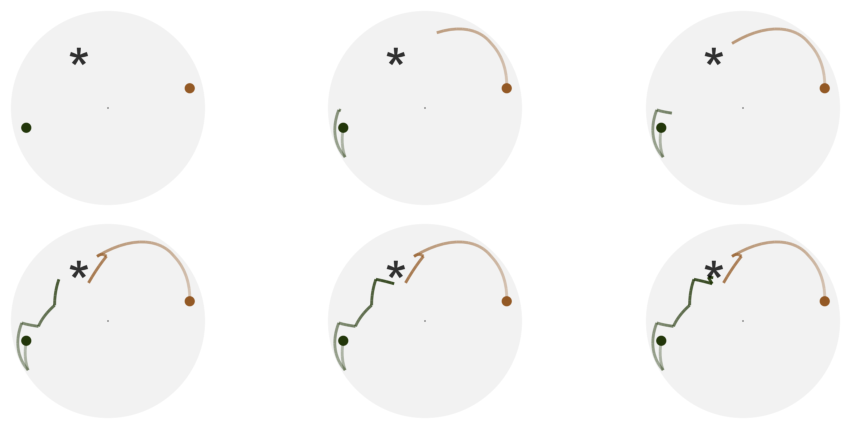
\includegraphics[width=1\linewidth]{figs/toy-pca-animated-1} 

}

\caption{Six frames selected from the animated version of the previous plot. With animation, the progression of the search paths from start to finish is better identified. CRS (green) finishes the optimisation quicker than PD (brown) since there is no further movement for CRS in the sixth frame. The full video of the animation can be found in the html version of the paper.}\label{fig:toy-pca-animated}
\end{figure}

\hypertarget{diagnostic-4a-the-tour-looking-at-itself}{%
\subsection{Diagnostic 4a: The tour looking at itself}\label{diagnostic-4a-the-tour-looking-at-itself}}

As mentioned previously, the original \(p \times d\) dimension space can be simulated via randomly generated bases in the \pkg{geozoo} (Schloerke 2016) package. While the PCA plot projects the bases from the direction that maximises the variance, the tour plot displays the original high-dimensional space from various directions using animation. Figure \ref{fig:toy-tour} shows some frames from the tour plot of the same two optimisations in its original space.

\begin{figure}

{\centering 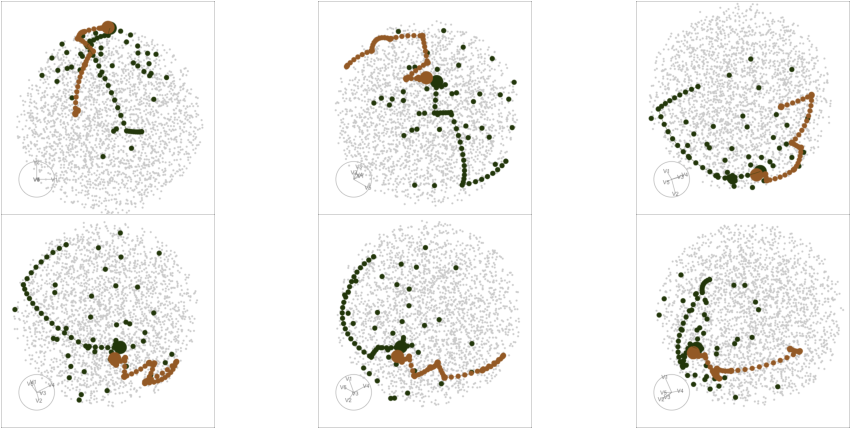
\includegraphics[width=1\linewidth]{figs/toy-tour-1} 

}

\caption{Six frames selected from rotating the high-dimensional basis space, along with the same two search paths from Figure \ref{fig:toy-pca} and \ref{fig:toy-pca-animated}. The basis space in this example is a 5D unit sphere, on which points (grey) are randomly generated via the CRAN package geozoo. The full animation can be seen in the html version of the paper.}\label{fig:toy-tour}
\end{figure}

\hypertarget{diagnostic-4b-forming-a-torus}{%
\subsection{Diagnostic 4b: Forming a torus}\label{diagnostic-4b-forming-a-torus}}

While the previous few examples have looked at the space of 1D basis in a unit sphere, this section visualises the space of 2D basis. Recall that the columns in a 2D basis are orthogonal to each other, so the space of \(p \times 2\) bases is a torus in the \(p\)-D space (Buja and Asimov 1986). For \(p = 3\) one would see a classical 3D torus shape as shown by the grey points in Figure \ref{fig:toy-torus}. The two circles of the torus can be observed to be perpendicular to each other and this can be linked back to the orthogonality condition. Two paths from CRS and PD are plotted on top of the torus and coloured in green and brown, respectively, to match the previous plots. The final basis found by PD and CRS are shown in a larger shape and printed below, respectively:

\begin{verbatim}
#>              [,1]        [,2]
#> [1,]  0.001196285  0.03273881
#> [2,] -0.242432715  0.96965761
#> [3,] -0.970167484 -0.24226493
\end{verbatim}

\begin{verbatim}
#>             [,1]         [,2]
#> [1,]  0.05707994 -0.007220138
#> [2,] -0.40196202 -0.915510160
#> [3,] -0.91387549  0.402230054
\end{verbatim}

Both optimisers have found the third variable in the first direction and the second variable in the second direction. Note, however, the different orientation of the basis, following from the different sign in the second column. One would expect to see this in the torus plot as the final bases match each other when projected onto one torus circle (due to the same sign in the first column) and are symmetric when projected onto the other (due to the different sign in the second column). In Figure \ref{fig:toy-torus}, this can be seen most clearly in frame 5 where the two circles are rotated into a line from our view.

\begin{figure}

{\centering 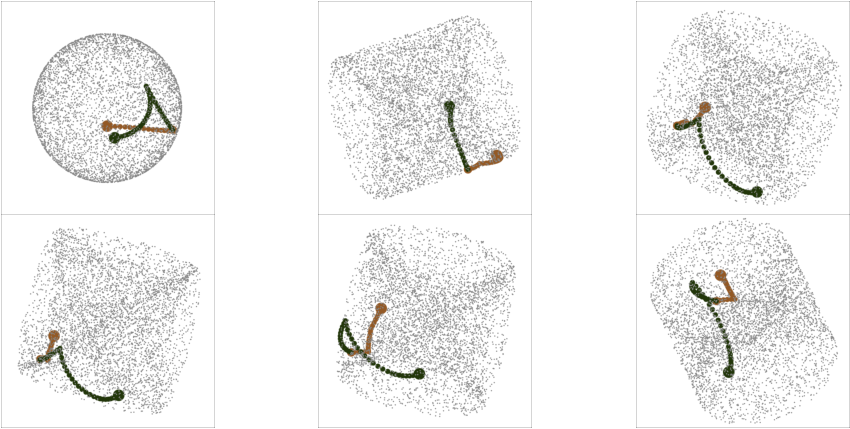
\includegraphics[width=1\linewidth]{figs/toy-torus-1} 

}

\caption{Six frames selected from rotating the 2D basis space along with two search paths optimised by PD (brown) and CRS (green). The projection problem is a 2D projection with three variables using the holes index. The grey points are randomly generated 2D projection bases in the space, and it can be observed that these points form a torus. The full video of the animation can be found in the html version of the paper.}\label{fig:toy-torus}
\end{figure}

\hypertarget{application}{%
\section{Diagnosing an optimiser}\label{application}}

In this section, several examples will be presented to show how the diagnostic plots discover something unexpected in projection pursuit optimisation, and guide the implementation of new features.

\hypertarget{simulation-setup}{%
\subsection{Simulation setup}\label{simulation-setup}}

Random variables with different distributions have been simulated as follows:

\begin{align}
x_1 \overset{d}{=} x_8 \overset{d}{=} x_9 \overset{d}{=} x_{10}& \sim \mathcal{N}(0, 1) \\
x_2 &\sim 0.5 \mathcal{N}(-3, 1) + 0.5 \mathcal{N}(3, 1)\\
\Pr(x_3) &= 
\begin{cases}
0.5 & \text{if $x_3 = -1$ or $1$}\\
0 & \text{otherwise}
\end{cases}\\
x_4 &\sim 0.25 \mathcal{N}(-3, 1) + 0.75 \mathcal{N}(3, 1)\\
x_5 &\sim \frac{1}{3} \mathcal{N}(-5, 1) + \frac{1}{3} \mathcal{N}(0, 1) + \frac{1}{3} \mathcal{N}(5, 1)\\
x_6 &\sim 0.45 \mathcal{N}(-5, 1) + 0.1 \mathcal{N}(0, 1) + 0.45 \mathcal{N}(5, 1)\\
x_7 &\sim 0.5 \mathcal{N}(-5, 1) + 0.5 \mathcal{N}(5, 1) 
\end{align}

\noindent Variables \texttt{x1}, \texttt{x8} to \texttt{x10} are normal noise with zero mean, and unit variance and \texttt{x2} to \texttt{x7} are normal mixtures with varied weights and locations. All the variables have been scaled to have overall unit variance before projection pursuit. The holes index (Dianne Cook et al. 2008), used for detecting bimodality of the variables, is used throughout the examples unless otherwise specified.

\hypertarget{monotonic}{%
\subsection{A problem of non-monotonicity}\label{monotonic}}

An example of non-monotonic interpolation has been given in Figure \ref{fig:toy-interp}: a path that passes bases with a higher index value than the target one. For SA, a non-monotonic interpolation is justified since target bases do not necessarily have a higher index value than the current one, while this is not the case for CRS. The original trace plot for a 2D projection problem, optimised by CRS, is shown on the left panel of Figure \ref{fig:interruption}, and one can observe that the non-monotonic interpolation has undermined the optimiser to realise its full potential. Hence, an interruption is implemented to stop at the best basis found in the interpolation. The right panel of Figure \ref{fig:interruption} shows the trace plot after implementing the interruption, and while the first two interpolations are identical, the basis at time 61 has a higher index value than the target in the third interpolation. Rather than starting the next iteration from the target basis on time 65, CRS starts the next iteration at time 61 on the right panel and reaches a better final basis.

\begin{figure}

{\centering \includegraphics[width=1\linewidth]{figs/interrupt} 

}

\caption{Comparison of the interpolation before and after implementing the interruption for the 2D projection problem on \code{boa6} data using holes index, optimised by CRS. On the left panel, the basis with a higher index value is found during the interpolation but not used. On the right panel, the interruption stops the interpolation at the basis with the highest index value for each iteration and results in a final basis with a higher index value, as shown on the right panel.}\label{fig:interruption}
\end{figure}

\hypertarget{close-but-not-close-enough}{%
\subsection{Close but not close enough}\label{close-but-not-close-enough}}

Once the final basis has been found by an optimiser, one may want to push further in the close neighbourhood to see if an even better basis can be found. A polish search takes the final basis of an optimiser as the start of a new guided tour to search for local improvements. The polish algorithm is similar to the CRS but with three distinctions: 1) a hundred rather than one candidate bases are generated each time in the inner loop; 2) the neighbourhood size is reduced in the inner loop, rather than in the outer loop; and 3) three more termination conditions have been added to ensure the new basis generated is distinguishable from the current one in terms of the distance in the space, the relative change in the index value, and neighbourhood size:

\begin{enumerate}
\def\labelenumi{\arabic{enumi})}
\tightlist
\item
  the distance between the basis found and the current needs to be larger than 1e-3;
\item
  the relative change of the index value needs to be larger than 1e-5; and
\item
  the alpha parameter needs to be larger than 0.01.
\end{enumerate}

Figure \ref{fig:polish} presents the projected data and trace plot of a 2D projection, optimised by CRS and followed by the polish step. The top row shows the initial projection, the final projection after CRS, and the final projection after polish, respectively. The end basis found by CRS reveals the four clusters in the data, but the edges of each cluster are not clean-cut. Polish works with this end basis and further pushes the index value to produce clearer edges of the cluster, especially along the vertical axis.

\begin{figure}

{\centering \includegraphics[width=1\linewidth]{figs/polish} 

}

\caption{Comparison of the projected data before and after using polishing for a 2D projection problem on \code{boa6} data using holes index. The top row shows the initial projected data and the final views after CRS and polish search, and the second row traces the index value. The clustering structure in the data is detected by CRS (top middle panel), but the polish step improves the index value and produces clearer boundaries of the clusters (top right panel), especially along the vertical axis. Note that the parameter \code{max.tries} is set to 400 in this experiment for CRS to do its best.}\label{fig:polish}
\end{figure}

\hypertarget{seeing-the-signal-in-the-noise}{%
\subsection{Seeing the signal in the noise}\label{seeing-the-signal-in-the-noise}}

The holes index function used for all the examples before this section produces a smooth interpolation, while this is not the case for all the indexes. An example of a noisy index function for 1D projections compares the projected data, \(\mathbf{Y}_{n \times 1}\), to a randomly generated normal distribution, \(\mathcal{N}_{n \times 1}\), using the Kolmogorov test. Let \(F_{.}(n)\) be the empirical cumulative distribution function (ECDF) with two possible subscripts, \(Y\) and \(\mathcal{N}\), representing the projected and randomly generated data, and \(n\) denoting the number of observations, the Kolmogorov index \(I^{nk}(n)\), is defined as:

\[I^{K}(n) = \max \left[F_{Y}(n) - F_{\mathcal{N}}(n)\right].\] With a non-smooth index function, two research questions are raised:

\begin{enumerate}
\def\labelenumi{\arabic{enumi})}
\tightlist
\item
  whether any optimiser fails to optimise this non-smooth index; and
\item
  whether the optimisers can find the global optimum despite the presence of a local optimum.
\end{enumerate}

Figure \ref{fig:noisy-better-geo} presents the trace and PCA plots of all three optimisers, and as expected, none of the interpolated paths are smooth. There is barely any improvement made by PD, indicating its failure in optimising non-smooth index functions. While CRS and SA have managed to get close to the index value of the theoretical best, the trace plot shows that it takes SA much longer to find the final basis. This long interpolation path is partially due to the fluctuation in the early iterations, where SA tends to generously accept inferior bases before concentrating near the optimum. The PCA plot shows the interpolation path and search points, excluding the last termination iteration. Pseudo-Derivative (PD) quickly gets stuck near the starting position. Comparing the amount of random search done by CRS and SA, it is surprising that SA does not carry as many samples as CRS. Combining the insights from both the trace and PCA plot, one can learn the two different search strategies by CRS and SA: CRS frequently samples in the space and only make a move when an improvement is guaranteed to be made, while SA first broadly accepts bases in the space and then starts the extensive sampling in a narrowed subspace. The specific decision of which optimiser to use will depend on the index curve in the basis space, but if the basis space is non-smooth, accepting inferior bases at first, as SA has done here, can lead to a more efficient search in terms of the overall number of points evaluated.

\begin{figure}

{\centering \includegraphics[width=1\linewidth]{figs/noisy-better-geo} 

}

\caption{Comparison of the three optimisers in optimising $I^{nk}(n)$ index for a 1D projection problem on a five-variable dataset, \code{boa5}. Both CRS and SA succeed in the optimisation, PD fails to optimise this non-smooth index. Further, SA takes  much longer than CRS to finish the optimisation, but finishes off closer to the theoretical best.}\label{fig:noisy-better-geo}
\end{figure}

The next experiment compares the performance of CRS and SA when a local maximum exists. Two search neighbourhood sizes, 0.5 and 0.7, are compared to understand how a large search neighbourhood would affect the final basis and the length of the search. Figure \ref{fig:kol-result} shows 80 paths simulated using 20 seeds in the PCA plot, faceted by the optimiser and search size. With CRS and a search size of 0.5, despite being the simplest and fastest, the optimiser fails in three instances where the final basis lands neither near the local nor the global optimum. With a larger search size of 0.7, more seeds have found the global maximum. Comparing CRS and SA for a search size of 0.5, SA does not seem to improve the final basis found, despite having longer interpolation paths. However, the denser paths near the local maximum are an indicator that SA is working hard to examine if there is any other optimum in the basis space, but the relatively small search size has diminished its ability to reach the global maximum. With a larger search size, almost all the seeds (16 out of 20) have found the global maximum, and some final bases are much closer to the theoretical best, as compared to the three other cases. This indicates that SA, with a reasonable large search window, is able to overcome the local optimum and optimise close towards the global optimum.

\begin{figure}

{\centering \includegraphics[width=1\linewidth]{figs/kol-result} 

}

\caption{Comparing 20 search paths in the PCA-projected basis space faceted by two optimisers: CRS and SA, and two search sizes: 0.5 and 0.7. The optimisation is on the 1D projection index, $I^{nk}(n)$, for \code{boa6} data, where a local optimum, annotated by the cross (x), is presented in this experiment, along with the global optimum (*).}\label{fig:kol-result}
\end{figure}

\hypertarget{reconciling-the-orientation}{%
\subsection{Reconciling the orientation}\label{reconciling-the-orientation}}

One interesting situation observed in the previous examples is that, for some simulations, as shown on the left panel of Figure \ref{fig:flip-sign}, the target basis is generated on the other half of the basis space, and the interpolator seems to draw a straight line to interpolate. Bases with opposite signs do not affect the projection and index value, but we would prefer the target to have the same orientation as the current basis. The orientation of two bases can be computationally checked by calculating the determinant -- a negative value suggests the two bases have a different orientation. For 1D bases, this can be corrected by flipping the sign on one basis. For higher dimensions, it can be a bit more difficult because the orthonormality of the basis needs to be also maintained when an individual vector is flipped. Here, an orientation check is carried out once a new target basis is generated, and the sign in the target basis will be flipped if a negative determinant is obtained. The interpolation after implementing the orientation check is shown on the right panel of Figure \ref{fig:flip-sign}, where the unsatisfactory interpolation no longer exists.

\begin{figure}

{\centering \includegraphics[width=1\linewidth]{figs/flip-sign} 

}

\caption{Comparison of the interpolation in the PCA-projected basis space before and after reconciling the orientation of the target basis. Optimisation is on the 1D projection index, $I^{nk}(n)$, for boa6 data using CRS with seed 2463. The dots represent the target basis in each iteration, and the path shows the interpolation. On the left panel, one target basis is generated with an opposite orientation to the current basis (hence appear on the other side of the basis space), and the interpolator crosses the origin to perform the interpolation. The right panel shows the same interpolation after implementing an orientation check, and the undesirable interpolation disappears.}\label{fig:flip-sign}
\end{figure}

\hypertarget{implementation}{%
\section{Implementation}\label{implementation}}

This project contributes to the software development in two packages: a data collection object is implemented in \pkg{tourr} (H. Wickham et al. 2011), while the visual diagnostics of the optimisers is implemented in \pkg{ferrn} (Zhang et al. 2021). The functions in the \pkg{ferrn} (Zhang et al. 2021) package are listed below:

\begin{itemize}
\item
  Main plotting functions:

  \begin{itemize}
  \tightlist
  \item
    \texttt{explore\_trace\_search()} produces summary plots in Figure \ref{fig:toy-search}.
  \item
    \texttt{explore\_trace\_interp()} produces trace plots for the interpolation points in Figure \ref{fig:toy-interp}.
  \item
    \texttt{explore\_space\_pca()} produces the PCA plot of projection bases on the reduced space. Figure \ref{fig:toy-pca} includes the additional details of anchor and search bases, which can be turned on by the argument \texttt{details\ =\ TRUE}. The animated version in Figure \ref{fig:toy-pca-animated} is produced with argument \texttt{animate\ =\ TRUE}.
  \item
    \texttt{explore\_space\_tour()} produces animated tour view on the full space of the projection bases in Figure \ref{fig:toy-tour}.
  \end{itemize}
\item
  \texttt{get\_*()} extracts and manipulates certain components from the existing data object.

  \begin{itemize}
  \tightlist
  \item
    \texttt{get\_anchor()} extracts target observations.
  \item
    \texttt{get\_basis\_matrix()} flattens all the bases into a matrix.
  \item
    \texttt{get\_best()} extracts the observation with the highest index value in the data object.
  \item
    \texttt{get\_dir\_search()} extracts directional search observations for PD search.
  \item
    \texttt{get\_interp()} extracts interpolated observations.
  \item
    \texttt{get\_interp\_last()} extracts the ending interpolated observations in each iteration.
  \item
    \texttt{get\_interrupt()} extracts the ending interpolated observations and the target observations if the interpolation is .interrupted
  \item
    \texttt{get\_search()} extracts search observations.
  \item
    \texttt{get\_search\_count()} extracts the count of search observations.
  \item
    \texttt{get\_space\_param()} produces the coordinates of the centre and radius of the basis space.
  \item
    \texttt{get\_start()} extracts the starting observation.
  \item
    \texttt{get\_theo()} extracts the theoretical best observations, if given.
  \end{itemize}
\item
  \texttt{bind\_*()} incorporates additional information outside the tour optimisation into the data object.

  \begin{itemize}
  \tightlist
  \item
    \texttt{bind\_theoretical()} binds the theoretical best observation in simulated experiment.
  \item
    \texttt{bind\_random()} binds randomly generated bases in the projection bases space to the data object.
  \item
    \texttt{bind\_random\_matrix()} binds randomly generated bases and outputs in a matrix format.
  \end{itemize}
\item
  \texttt{add\_*()} provides wrapper functions to create ggprotos for different components for the PCA plot

  \begin{itemize}
  \tightlist
  \item
    \texttt{add\_anchor()} for plotting anchor bases.
  \item
    \texttt{add\_anno()} for annotating the symmetry of start bases.
  \item
    \texttt{add\_dir\_search()} for plotting the directional search bases with magnified distance.
  \item
    \texttt{add\_end()} for plotting end bases.
  \item
    \texttt{add\_interp()} for plotting the interpolation path.
  \item
    \texttt{add\_interp\_last()} for plotting the last interpolation bases for comparing with target bases when interruption is used.
  \item
    \texttt{add\_interrupt()} for linking the last interpolation bases with target ones when interruption is used.
  \item
    \texttt{add\_search()} for plotting search bases.
  \item
    \texttt{add\_space()} for plotting the circular space.
  \item
    \texttt{add\_start()} for plotting start bases.
  \item
    \texttt{add\_theo()} for plotting theoretical best bases, if applicable.
  \end{itemize}
\item
  Utilities

  \begin{itemize}
  \tightlist
  \item
    \texttt{theme\_fern()} and \texttt{format\_label()} for better display of the grid lines and axis formatting.
  \item
    \texttt{clean\_method()} to clean up the name of the optimisers.
  \item
    \texttt{botanical\_palettes()} is a collection of colour palettes from Australian native plants. Quantitative palettes include daisy, banksia, and cherry, and sequential palettes contain fern and acacia.
  \item
    \texttt{botanical\_pal()} as the colour interpolator.
  \item
    \texttt{scale\_color\_*()} and \texttt{scale\_fill\_*()} for scaling the colour and fill of the plot.
  \end{itemize}
\end{itemize}

\hypertarget{conclusion}{%
\section{Conclusion}\label{conclusion}}

This paper has provided several visual diagnostics that can be used for understanding a complex optimisation procedure and are implemented in the \textbf{ferrn} package. The methods were illustrated using the optimisers available for projection pursuit guided tour. Here the constraint is the orthonormality condition of the projection bases, which corresponds to optimisation over spheres and torii. The approach described broadly applies to other constrained optimisers. Although the manifold in \(p\)-space might be different the diagnostic techniques are the same. A researcher would begin by saving the path of the optimiser in a form required to input into the ferrn package, as described in this paper. One might generally make more samples from the constrained space upon which to assess and compare the optimisation paths. These high-dimensional data objects can then be viewed using the tour.

The progressive optimisation of a target function and its coverage of the search space can be viewed in both reduced 2D space and the full space. These visualisations can lead to insights for evaluating and comparing the performance of multiple optimisers operating on the same task. They can provide a better understanding of existing methods or motivate the development of new approaches. For example, we have compared how three optimisers perform when maximising a non-smooth index function and have illustrated how the pseudo-derivative search fails in this setting. The observations from our experiments have also been translated into improved optimisation methods for the guided tour, e.g., we introduced the option to interrupt the search if a better basis is found along the path.

This work might be considered an effort to bring transparency into algorithms. Although little attention is paid by algorithm developers to providing ways to output information during intermediate steps, this is an important component for enabling others to understand and diagnose the performance. Algorithms are an essential component of artificial intelligence that is used to make daily life easier. Interpretability of algorithms is important to guard against aspects like bias and inappropriate use. The data object underlying the visual diagnostics here is an example of what might be useful in algorithm development generally.

\hypertarget{acknowledgements}{%
\section{Acknowledgements}\label{acknowledgements}}

This article is created using \CRANpkg{knitr} (Xie 2015) and \CRANpkg{rmarkdown} (Xie, Allaire, and Grolemund 2018) in R. The source code for reproducing this paper can be found at: \url{https://github.com/huizezhang-sherry/paper-ferrn}.

\hypertarget{references}{%
\section*{References}\label{references}}
\addcontentsline{toc}{section}{References}

\hypertarget{refs}{}
\begin{CSLReferences}{1}{0}
\leavevmode\vadjust pre{\hypertarget{ref-andradottir2015review}{}}%
Andradóttir, Sigrún. 2015. {``A Review of Random Search Methods.''} In \emph{Handbook of Simulation Optimization}, 277--92. Springer. \url{https://doi.org/10.1007/978-1-4939-1384-8}.

\leavevmode\vadjust pre{\hypertarget{ref-bertsekas2014constrained}{}}%
Bertsekas, Dimitri P. 2014. \emph{Constrained Optimization and Lagrange Multiplier Methods}. Academic press. \url{https://doi.org/10.1016/C2013-0-10366-2}.

\leavevmode\vadjust pre{\hypertarget{ref-bertsimas1993simulated}{}}%
Bertsimas, Dimitris, and John Tsitsiklis. 1993. {``Simulated Annealing.''} \emph{Statistical Science} 8 (1): 10--15. \url{https://doi.org/10.1214/ss/1177011077}.

\leavevmode\vadjust pre{\hypertarget{ref-Brooks1958-zk}{}}%
Brooks, Samuel H. 1958. {``A Discussion of Random Methods for Seeking Maxima.''} \emph{Operations Research} 6 (2): 244--51. \url{https://doi.org/10.1287/opre.6.2.244}.

\leavevmode\vadjust pre{\hypertarget{ref-Buja1986-sw}{}}%
Buja, Andreas, and Daniel Asimov. 1986. {``Grand Tour Methods: An Outline.''} In \emph{Proceedings of the Seventeenth Symposium on the Interface of Computer Sciences and Statistics}, 63--67. USA: Elsevier North-Holland, Inc. \url{https://dl.acm.org/doi/10.5555/26036.26046}.

\leavevmode\vadjust pre{\hypertarget{ref-buja2005computational}{}}%
Buja, Andreas, Dianne Cook, Daniel Asimov, and Catherine Hurley. 2005. {``Computational Methods for High-Dimensional Rotations in Data Visualization.''} \emph{Handbook of Statistics} 24: 391--413. \url{https://doi.org/10.1016/S0169-7161(04)24014-7}.

\leavevmode\vadjust pre{\hypertarget{ref-conn2009introduction}{}}%
Conn, Andrew R, Katya Scheinberg, and Luis N Vicente. 2009. \emph{Introduction to Derivative-Free Optimization}. SIAM. \url{https://doi.org/10.1137/1.9780898718768}.

\leavevmode\vadjust pre{\hypertarget{ref-cook1993projection}{}}%
Cook, D., A. Buja, and J. Cabrera. 1993. {``Projection Pursuit Indexes Based on Orthonormal Function Expansions.''} \emph{Journal of Computational and Graphical Statistics} 2 (3): 225--50. \url{https://doi.org/10.2307/1390644}.

\leavevmode\vadjust pre{\hypertarget{ref-cook1997manual}{}}%
Cook, Dianne, and Andreas Buja. 1997. {``Manual Controls for High-Dimensional Data Projections.''} \emph{Journal of Computational and Graphical Statistics} 6 (4): 464--80. \url{https://doi.org/10.2307/1390747}.

\leavevmode\vadjust pre{\hypertarget{ref-cook1995grand}{}}%
Cook, Dianne, Andreas Buja, Javier Cabrera, and Catherine Hurley. 1995. {``Grand Tour and Projection Pursuit.''} \emph{Journal of Computational and Graphical Statistics} 4 (3): 155--72. \url{https://doi.org/10.1080/10618600.1995.10474674}.

\leavevmode\vadjust pre{\hypertarget{ref-cook2008grand}{}}%
Cook, Dianne, Andreas Buja, Eun-Kyung Lee, and Hadley Wickham. 2008. {``Grand Tours, Projection Pursuit Guided Tours, and Manual Controls.''} In \emph{Handbook of Data Visualization}, 295--314. Springer. \url{https://doi.org/10.1007/978-3-540-33037-0_13}.

\leavevmode\vadjust pre{\hypertarget{ref-diaconis1984asymptotics}{}}%
Diaconis, Persi, and David Freedman. 1984. {``Asymptotics of Graphical Projection Pursuit.''} \emph{The Annals of Statistics}, 793--815. \url{https://doi.org/10.1214/aos/1176346703}.

\leavevmode\vadjust pre{\hypertarget{ref-friedman1974projection}{}}%
Friedman, Jerome H, and John W Tukey. 1974. {``A Projection Pursuit Algorithm for Exploratory Data Analysis.''} \emph{IEEE Transactions on Computers} 100 (9): 881--90. \url{https://doi.org/10.1109/T-C.1974.224051}.

\leavevmode\vadjust pre{\hypertarget{ref-granville1994simulated}{}}%
Granville, Vincent, Mirko Krivánek, and J-P Rasson. 1994. {``Simulated Annealing: A Proof of Convergence.''} \emph{IEEE Transactions on Pattern Analysis and Machine Intelligence} 16 (6): 652--56. \url{https://doi.org/10.1109/34.295910}.

\leavevmode\vadjust pre{\hypertarget{ref-hall1989polynomial}{}}%
Hall, Peter. 1989. {``On Polynomial-Based Projection Indices for Exploratory Projection Pursuit.''} \emph{The Annals of Statistics} 17 (2): 589--605. \url{https://doi.org/10.1214/aos/1176347127}.

\leavevmode\vadjust pre{\hypertarget{ref-healy2018data}{}}%
Healy, Kieran. 2018. \emph{Data Visualization: A Practical Introduction}. Princeton University Press. \url{https://socviz.co/}.

\leavevmode\vadjust pre{\hypertarget{ref-jones1998efficient}{}}%
Jones, Donald R, Matthias Schonlau, and William J Welch. 1998. {``Efficient Global Optimization of Expensive Black-Box Functions.''} \emph{Journal of Global Optimization} 13 (4): 455--92. \url{https://doi.org/10.1023/A:1008306431147}.

\leavevmode\vadjust pre{\hypertarget{ref-kirkpatrick1983optimization}{}}%
Kirkpatrick, Scott, C Daniel Gelatt, and Mario P Vecchi. 1983. {``Optimization by Simulated Annealing.''} \emph{Science} 220 (4598): 671--80. \url{https://doi.org/10.1126/science.220.4598.671}.

\leavevmode\vadjust pre{\hypertarget{ref-laa2020using}{}}%
Laa, Ursula, and Dianne Cook. 2020. {``Using Tours to Visually Investigate Properties of New Projection Pursuit Indexes with Application to Problems in Physics.''} \emph{Computational Statistics}, 1--35. \url{https://doi.org/10.1007/s00180-020-00954-8}.

\leavevmode\vadjust pre{\hypertarget{ref-lee2005projection}{}}%
Lee, E., D. Cook, S. Klinke, and T. Lumley. 2005. {``Projection Pursuit for Exploratory Supervised Classification.''} \emph{Journal of Computational and Graphical Statistics} 14 (4): 831--46. \url{https://doi.org/10.1198/106186005X77702}.

\leavevmode\vadjust pre{\hypertarget{ref-lee2010projection}{}}%
Lee, Eun-Kyung, and Dianne Cook. 2010. {``A Projection Pursuit Index for Large p Small n Data.''} \emph{Statistics and Computing} 20 (3): 381--92. \url{https://doi.org/10.1007/s11222-009-9131-1}.

\leavevmode\vadjust pre{\hypertarget{ref-li2020visualizing}{}}%
Li, Mingwei, Zhenge Zhao, and Carlos Scheidegger. 2020. {``Visualizing Neural Networks with the Grand Tour.''} \emph{Distill}. \url{https://doi.org/10.23915/distill.00025}.

\leavevmode\vadjust pre{\hypertarget{ref-Loperfido2018}{}}%
Loperfido, Nicola. 2018. {``Skewness-Based Projection Pursuit: A Computational Approach.''} \emph{Computational Statistics and Data Analysis} 120 (C): 42--57. \url{https://doi.org/10.1016/j.csda.2017.11.001}.

\leavevmode\vadjust pre{\hypertarget{ref-Loperfido2020}{}}%
---------. 2020. {``Kurtosis-Based Projection Pursuit for Outlier Detection in Financial Time Series.''} \emph{The European Journal of Finance} 26 (2-3): 142--64. \url{https://doi.org/10.1080/1351847X.2019.1647864}.

\leavevmode\vadjust pre{\hypertarget{ref-mitra1986convergence}{}}%
Mitra, Debasis, Fabio Romeo, and Alberto Sangiovanni-Vincentelli. 1986. {``Convergence and Finite-Time Behavior of Simulated Annealing.''} \emph{Advances in Applied Probability} 18 (3): 747--71. \url{https://doi.org/10.1109/CDC.1985.268600}.

\leavevmode\vadjust pre{\hypertarget{ref-posse1995projection}{}}%
Posse, Christian. 1995. {``Projection Pursuit Exploratory Data Analysis.''} \emph{Computational Statistics \& Data Analysis} 20 (6): 669--87. \url{https://doi.org/10.1016/0167-9473(95)00002-8}.

\leavevmode\vadjust pre{\hypertarget{ref-rios2013derivative}{}}%
Rios, Luis Miguel, and Nikolaos V Sahinidis. 2013. {``Derivative-Free Optimization: A Review of Algorithms and Comparison of Software Implementations.''} \emph{Journal of Global Optimization} 56 (3): 1247--93. \url{https://doi.org/10.1007/s10898-012-9951-y}.

\leavevmode\vadjust pre{\hypertarget{ref-Romeijn2009}{}}%
Romeijn, H. Edwin. 2009. {``Random Search Methods.''} In \emph{Encyclopedia of Optimization}, 3245--51. Boston, MA: Springer US. \url{https://doi.org/10.1007/978-0-387-74759-0_556}.

\leavevmode\vadjust pre{\hypertarget{ref-geozoo}{}}%
Schloerke, Barret. 2016. \emph{Geozoo: Zoo of Geometric Objects}. \url{https://CRAN.R-project.org/package=geozoo}.

\leavevmode\vadjust pre{\hypertarget{ref-spall2005introduction}{}}%
Spall, James C. 2005. \emph{Introduction to Stochastic Search and Optimization: Estimation, Simulation, and Control}. Vol. 65. John Wiley \& Sons. \url{https://www.jhuapl.edu/ISSO/}.

\leavevmode\vadjust pre{\hypertarget{ref-tukey1977exploratory}{}}%
Tukey, John W. 1977. \emph{Exploratory Data Analysis}. Vol. 2. Reading, MA.

\leavevmode\vadjust pre{\hypertarget{ref-unwin2015graphical}{}}%
Unwin, Antony. 2015. \emph{Graphical Data Analysis with r}. Vol. 27. CRC Press. \url{https://doi.org/10.1201/9781315370088}.

\leavevmode\vadjust pre{\hypertarget{ref-White1971-ci}{}}%
White, R C. 1971. {``A Survey of Random Methods for Parameter Optimization.''} \emph{Simulation} 17 (5): 197--205. \url{https://doi.org/10.1177/003754977101700504}.

\leavevmode\vadjust pre{\hypertarget{ref-wickham2014tidy}{}}%
Wickham, Hadley. 2014. {``Tidy Data.''} \emph{Journal of Statistical Software} 59 (10): 1--23. \url{https://doi.org/10.18637/jss.v059.i10}.

\leavevmode\vadjust pre{\hypertarget{ref-ggplot2}{}}%
---------. 2016. \emph{Ggplot2: Elegant Graphics for Data Analysis}. Springer-Verlag New York. \url{https://doi.org/10.1007/978-0-387-98141-3}.

\leavevmode\vadjust pre{\hypertarget{ref-dplyr}{}}%
Wickham, Hadley, Romain François, Lionel Henry, and Kirill Müller. 2020. \emph{Dplyr: A Grammar of Data Manipulation}. \url{https://CRAN.R-project.org/package=dplyr}.

\leavevmode\vadjust pre{\hypertarget{ref-tourr}{}}%
Wickham, H., D. Cook, H. Hofmann, and A. Buja. 2011. {``{tourr}: An {R} Package for Exploring Multivariate Data with Projections.''} \emph{Journal of Statistical Software} 40 (2): 1--18. \url{http://doi.org/10.18637/jss.v040.i02}.

\leavevmode\vadjust pre{\hypertarget{ref-wilke2019fundamentals}{}}%
Wilke, Claus O. 2019. \emph{Fundamentals of Data Visualization: A Primer on Making Informative and Compelling Figures}. O{'}Reilly Media. \url{https://clauswilke.com/dataviz/}.

\leavevmode\vadjust pre{\hypertarget{ref-scag}{}}%
Wilkinson, L., A. Anand, and R. Grossman. 2005. {``Graph-Theoretic Scagnostics.''} In \emph{IEEE Symposium on Information Visualization, 2005. INFOVIS 2005.}, 157--64.

\leavevmode\vadjust pre{\hypertarget{ref-WW08}{}}%
Wilkinson, Leland, and Graham Wills. 2008. {``Scagnostics Distributions.''} \emph{Journal of Computational and Graphical Statistics} 17 (2): 473--91.

\leavevmode\vadjust pre{\hypertarget{ref-knitr}{}}%
Xie, Yihui. 2015. \emph{Dynamic Documents with {R} and Knitr}. 2nd ed. Boca Raton, Florida: Chapman; Hall/CRC. \url{https://yihui.name/knitr/}.

\leavevmode\vadjust pre{\hypertarget{ref-rmarkdown}{}}%
Xie, Yihui, J. J. Allaire, and Garrett Grolemund. 2018. \emph{R Markdown: The Definitive Guide}. Boca Raton, Florida: Chapman; Hall/CRC. \url{https://bookdown.org/yihui/rmarkdown}.

\leavevmode\vadjust pre{\hypertarget{ref-zabinsky2013stochastic}{}}%
Zabinsky, Zelda B. 2013. \emph{Stochastic Adaptive Search for Global Optimization}. Vol. 72. Springer Science \& Business Media. \url{https://doi.org/10.1007/978-1-4419-9182-9}.

\leavevmode\vadjust pre{\hypertarget{ref-ferrn}{}}%
Zhang, H. Sherry, Dianne Cook, Ursula Laa, Nicolas Langrené, and Patricia Menéndez. 2021. \emph{Ferrn: Facilitate Exploration of touRR optimisatioN}. \url{https://github.com/huizezhang-sherry/ferrn/}.

\end{CSLReferences}

\bibliography{zhang-cook-laa-langrene-menendez.bib}

\address{%
H. Sherry Zhang\\
Monash University\\%
Department of Econometrics and Business Statistics\\ Melbourne, Australia\\
%
%
%
\href{mailto:huize.zhang@monash.edu}{\nolinkurl{huize.zhang@monash.edu}}%
}

\address{%
Dianne Cook\\
Monash University\\%
Department of Econometrics and Business Statistics\\ Melbourne, Australia\\
%
%
%
\href{mailto:dicook@monash.edu}{\nolinkurl{dicook@monash.edu}}%
}

\address{%
Ursula Laa\\
University of Natural Resources and Life Sciences\\%
Institute of Statistics\\ Vienna, Austria\\
%
%
%
\href{mailto:ursula.laa@boku.ac.at}{\nolinkurl{ursula.laa@boku.ac.at}}%
}

\address{%
Nicolas Langrené\\
CSIRO Data61\\%
34 Village Street, Docklands VIC 3008 Australia\\ Melbourne, Australia\\
%
%
%
\href{mailto:nicolas.langrene@csiro.au}{\nolinkurl{nicolas.langrene@csiro.au}}%
}

\address{%
Patricia Menéndez\\
Monash University\\%
Department of Econometrics and Business Statistics\\ Melbourne, Australia\\
%
%
%
\href{mailto:patricia.menendez@monash.edu}{\nolinkurl{patricia.menendez@monash.edu}}%
}

\end{article}


\end{document}
